\chapter{Experiments and Results}
\label{ch:results}
\section{Introduction}
\label{sec:res_intro}
\paragraph{\textnormal{This chapter presents the evaluation of the proposed mapping system through a series of experiments conducted on both custom and public datasets. The custom dataset includes trajectories of varying lengths (long and short) captured in diverse settings, containing both indoor and outdoor environments. The aim is to assess the system's performance in terms of trajectory accuracy, loop closure effectiveness, map consistency, and computational efficiency.
}}
\section{Experimental Setup}
\label{sec:exp_setup}

\subsection{Hardware and Platform}
\label{sec:hw_platform}
\paragraph{\textnormal{The custom datasets were collected using the Hunter 2.0 mobile robot from AgileX Robotics, equipped with an Ouster OS1-128 LiDAR. The sensor provides 128 scan lines, a 360° horizontal field of view, and operates at 10 Hz. It also includes a built-in IMU, which was used for LIO odometry estimation. The extrinsic calibration between the ouster LiDAR and the IMU can be computed online with FAST-LIO2, however in our experiments we used identity for rotation with no translation. All data were recorded using ROS 2 bag files for both real-time and offline processing. For running the mapping system, both in real-time and during offline refinement, a separate computer was used. It featured an AMD Ryzen 7 CPU, NVIDIA RTX 3060 GPU, and 32 GB RAM, running Ubuntu 22.04 with ROS 2 Humble. All mapping modules were implemented in C++ to ensure real-time performance and efficient offline processing.
}}


\begin{figure}[h!]
	\centering
	\begin{subfigure}[t]{0.43\textwidth}
		\centering
		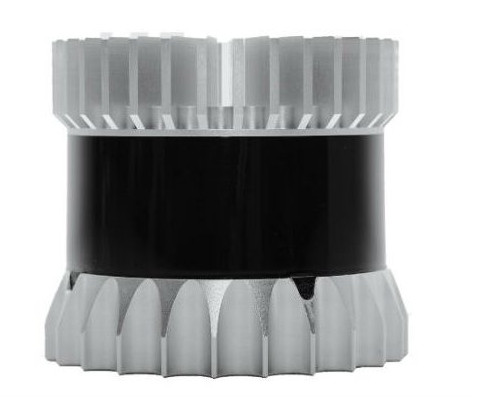
\includegraphics[width=\linewidth]{images/ouster_lidar.jpg}
		\caption{}
	\end{subfigure}
	\hfill
	\begin{subfigure}[t]{0.48\textwidth}
		\centering
		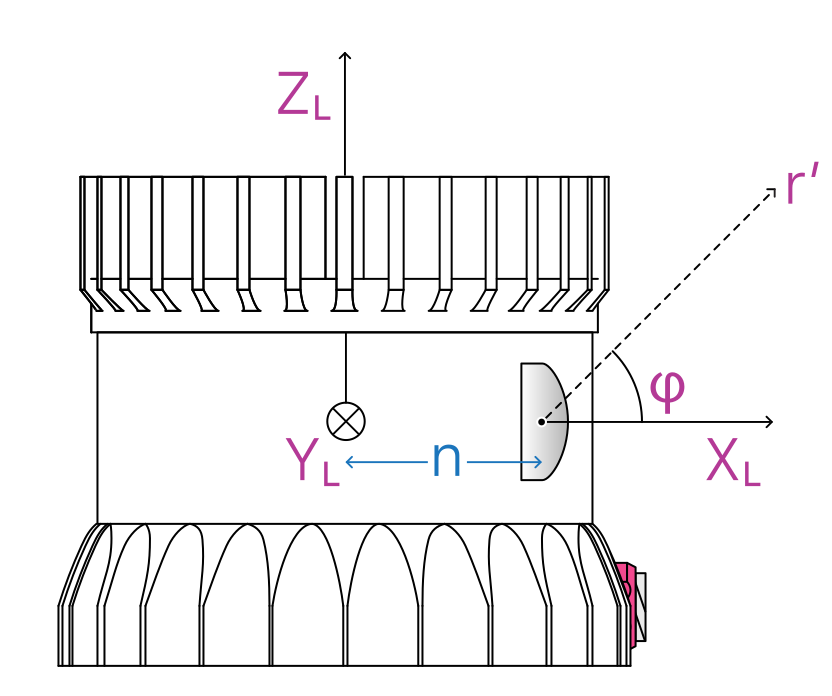
\includegraphics[width=\linewidth]{images/ouster_frame.png}
		\caption{}
	\end{subfigure}
	\caption{a) Ouster OS1-128 LiDAR with built-in IMU. b) Sensor coordinate frame \cite{ousterdocs}}
	\label{fig:overview}
\end{figure}

\subsection{Software Modules}
\label{sec:sw_modules}
\paragraph{\textnormal{The entire mapping pipeline contains modular components implemented in C++ within ROS2 Humble framework. The software dependencies of each components is summerized in table \ref{tab:sw_depends}. The version numbers we used in our experiments are shown in bold.
}}
\noindent
\begin{table}[H]
	\centering
	\caption{Software modules and dependencies}
	\begin{tabular}{|c|c|c|c|}
		\hline
		\diagbox{Deps}{Module} & FAST-LIO2 & PGO & HBA \\
		\hline
		C++ &\multicolumn{3}{c|}{17}  \\
		\hline
		Eigen &>=3.3.4(\textbf{3.4.0}) & \textbf{3.4.0} &>=3.3.7(\textbf{3.4.0})\\
		\hline
		GTSAM & None & \multicolumn{2}{c|}{>=4.1.1(\textbf{4.2.0})}\\
		\hline
		PCL &>=1.8(\textbf{1.12.1}) & \textbf{1.12.1} &>=1.10.0(\textbf{1.12.1}) \\
		\hline
		Ubuntu & \multicolumn{3}{c|}{22.04} \\
		\hline
		ROS & \multicolumn{3}{c|}{Humble} \\
		\hline
	\end{tabular}
	\label{tab:sw_depends}
\end{table}


\subsection{Dataset}
\label{sec:dataset}
\paragraph{\textnormal {To evaluate the performance of our mapping system, we performed experiments with various open source dataset and our own dataset collected around Saxion building. Experiments with the open source MulRan \cite{gskim-2020-mulran} and KITTI \cite{Geiger2013IJRR} dataset were performed to evaluate the robustness of our mapping module  to different variety of sensors types, seasonal and environmental changes. These open source dataset also contain ground truth trajectories that we used for comparing the performance of our method. The sequences KAIST02, KAIST03, and RiverSide01 from MulRan and sequences 00, and 05 from KITTI are used in the experimentation.}}

\noindent
\begin{table}[H]
	\centering
		\caption{Dataset used for evaluating performance of our mapping module}
	\begin{tabular}{ccccclclc}
		\toprule
		Dataset 	& 	LiDAR 	 		& Envt. 	& G.Truth		& Size &Dist.(m) & Duration(s)\\
		\midrule
		Saxion-01 	& OS-128 			& Outdoor	& \xmark		& 11GB &935			&740	\\
		Saxion-02 	& OS-128 			& Outdoor	& \xmark		& 29GB &1155 		&958	 \\
		Saxion-03 	& OS-128 			& Outdoor	& \xmark		& 50GB &1823 		&1668	 \\
		Saxion-11 	& OS-128 			& Indoor	& \xmark		& 54GB &431			&696	 \\
		KITTI05 	& HDL-64E 			& Outdoor	& \cmark		& 6GB &2205 		&288	 \\
		KAIST02 	& OS1-64 			& Outdoor	& \cmark		& 24GB &??? 		&894	 \\
		KAIST03 	& OS1-64 			& Outdoor	& \cmark		& 18GB &6272 		&862	 \\
		RiverSide01 & OS1-64 			& Outdoor	& \cmark		& 8GB &6272 		&535	 \\		
		
		\bottomrule& & 
	\end{tabular}
	\label{tab:datasets}
\end{table}
In order for the SLAM to work correctly for each dataset, an extrinsic calibration between the IMU and LiDAR sensors is required. Table \ref{tab:calibration} shows the calibration matrix for each dataset used in the experiments.
\noindent
\begin{table}[H]
	\centering
	\caption{Extrinsic calibration between IMU and LiDAR for the different datasets we used}
	\begin{tabular}{ccccclclc}
		\toprule
		Dataset 	& 	Rotation 	 		&Translation(x, y, z)\\
		\midrule
		Saxion 	& Identity 			& 0,	0,		0	\\
		KITTI 	& Identity 			& 0.81, -0.32, 0.8	\\
		KAIST 	& \(\begin{bmatrix}
			-1 & 0 & 0 \\
			0 & -1 & 0 \\
			0 & 0 & 1
		\end{bmatrix}\) 			& 1.77, 0.0, -0.05	\\
		\bottomrule& & 
	\end{tabular}
	\label{tab:calibration}
\end{table}
%\subsection{Analysis of Accuracy}
%\paragraph{\textnormal{Figure \ref{fig:kaist02} shows the result of the map and trajectory before and after applying optimization to the output of the LiDAR odometry based poses. It can be clearly seen in \ref{fig:odom_map} that the map generated by odometry is not accurate and it has duplication in most part of the map specially on the top right corner side.}}
%
%
%\paragraph{\textnormal{As initial step, we tested on the Mulran KAIST02 sequence using the odometry from FAST-LIO2 and generated map both from the odometry and pose-graph optimization.}}
%
%\paragraph{\textnormal{The map shown in \ref{fig:pgo_map} is generated after the FAST-LIO2 poses are optimized by ISAM2 after adding loop closure constraints to the factor graph. Since this map is generated from the optimized poses, the duplications are now removed and is more consistent than the previous map. The drift accumulated by FAST-LIO2 odometry can be seen in figure \ref{fig:odom_path} and figure \ref{fig:pgo_path} shows the trajectory after the drift is corrected with ISAM2.}}
%
%\begin{figure}[H]
%	\centering
%	\begin{subfigure}{0.4\textwidth}
%	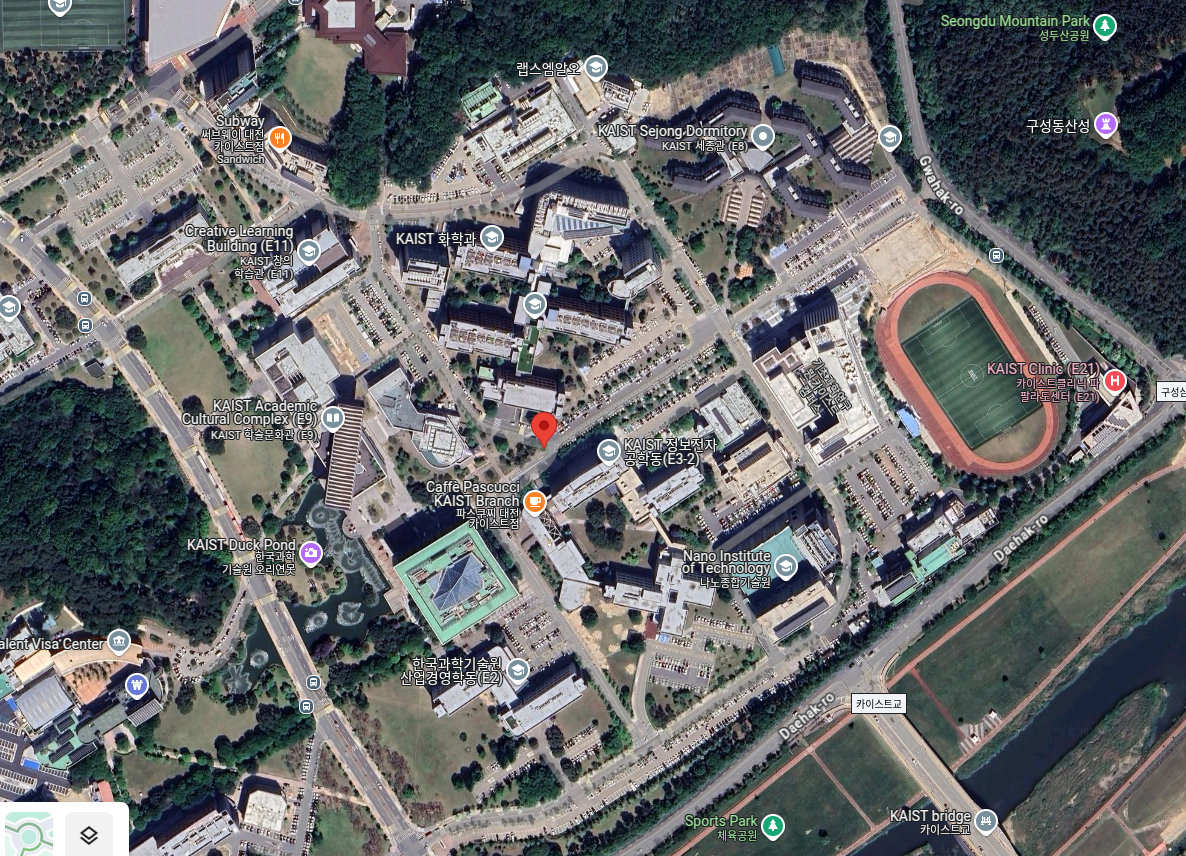
\includegraphics[width=\textwidth]{images/kaist_gmap.png}
%		\caption{KAIST google map}
%		\label{fig:odom_map}
%	\end{subfigure}
%	\begin{subfigure}{0.4\textwidth}
%	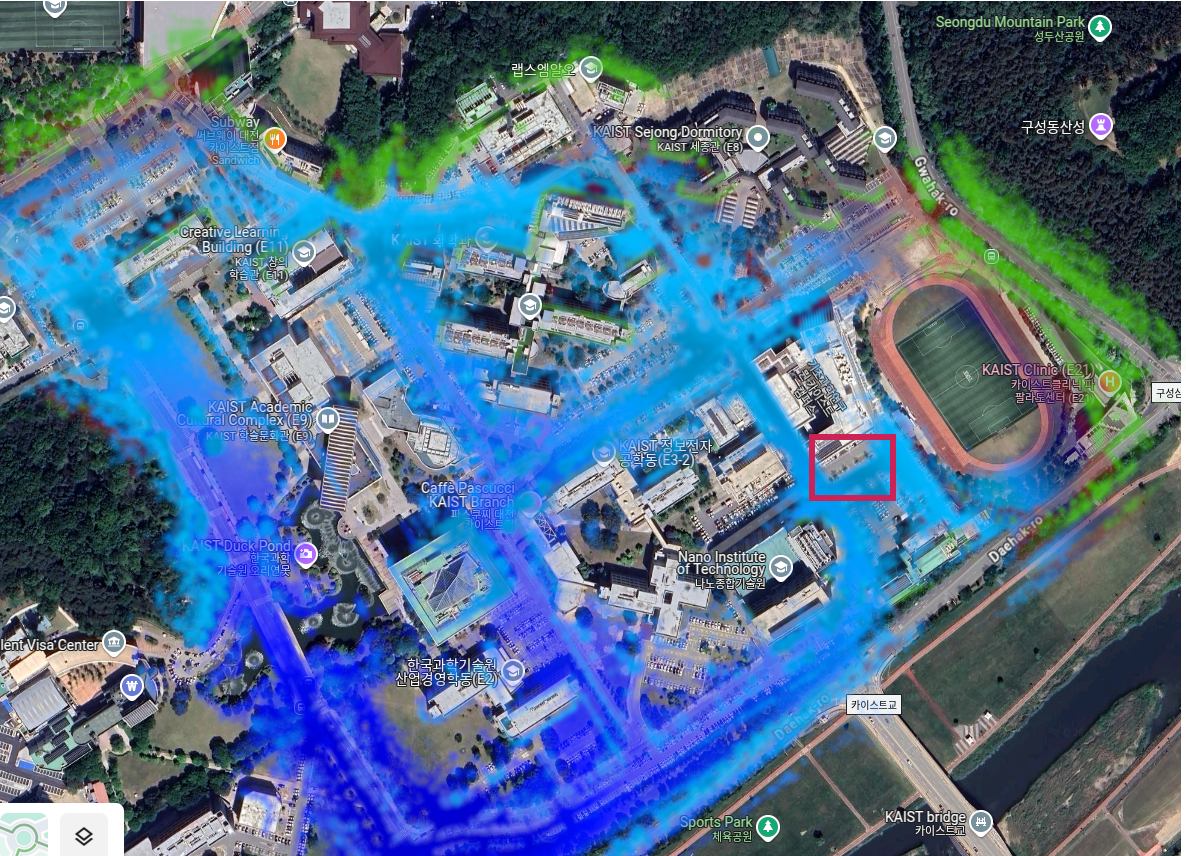
\includegraphics[width=\textwidth]{images/kaist02_gmap.png}
%	\caption{Map overlayed to google map}
%	\label{fig:odom_map}
%\end{subfigure}
%	\caption{Odometry showing direction of driving(not fully optimized because both optimization and publishing the odometry run in separate threads so the published odometry is not final optimized result)}
%\end{figure}
%\paragraph{\textnormal{To further analyze the accuracy of the optimized map, we overlayed the generated map onto the google map, and it can be seen that some small inconsistencies are visible because unlike LiDAR bundle adjustment methods \cite{bibid}, pose graph optimization does not optimize point cloud consistency directly\cite{pan2021mulls}. Instead, it focuses solely in optimizing relative pose errors. Hence the divergence is not completely eliminated in the map.}}
%% Things worth mentioning
%% - execution time
%\noindent
%\begin{table}[H]
%	\centering
%	\caption{Metric comparison of our SLAM with state-off-the-art for indoor custom indoor dataset at Saxion}
%	\begin{tabular}{clcccc}
%		\toprule
%		Method 			& 	avg runtime 	& avg freq. 	& 	Num loop closures\\
%		\midrule
%
%	 KISS-SLAM			& 	30ms			&	34.00 HZ			& 77\\
%	MOLA SLAM			&	29.72ms				&  	33.65HZ				& - \\
%	PROPOSED& &  & \\
%		\bottomrule
%
%	\end{tabular}
%	\label{tab:slam_comparison}
%\end{table}
%
%\paragraph{\textnormal{Table \ref{tab:slam_comparison} shows the comparison of our method with most recent SLAM methods, and it is shown that KISS-SLAM results in many false positive loop closures resulting inaccuracy in the generated map. The average runtime of both SLAM methods is comparably real-time.}}
%
\section{Evaluation metrics}
\label{sec:ev_metrics}
\paragraph{\textnormal{The proposed mapping pipeline was evaluated using a comprehensive set of quantitative and qualitative metrics to ensure a robust performance assessment. Specifically Absolute Pose Error(APE) was employed to evaluate the global consistency of the estimated trajectory by comparing it against the ground truth data. To measure local accuracy and drift between consecutive poses, Relative Pose Error (RPE) was employed. Map consistency was assessed qualitatively through visual inspection of the generated maps. Finally, Runtime Performance was measured by recording the average processing time per LiDAR scan in the online module. These evaluation criteria collectively provide a thorough insight into the accuracy, robustness, and efficiency of the developed system.}}



\section{Results}
\label{sec:results}
\paragraph{\textnormal{This section presents the results obtained from the proposed mapping system, including maps and trajectories generated using three components; FAST-LIO2 alone, FAST-LIO2 and PGO, and HBA for all the datasets mentioned in \ref{tab:datasets}. These results are analyzed to evaluate the accuracy and consistency of the mapping performance. For this purpose, we compare both the maps and the trajectories of the components in the mapping pipeline. 
}}
\subsection{Trajectory accuracy}
\paragraph{\textnormal{To evaluate the performance of the system, we compared trajectories generated by the three components for each dataset. For the KITTI and MulRan datasets, we compared the trajectories of our system with the ground truth trajctroy and computed the APE, and RPE. Since the custom datasets do not have ground truth trajectory, we used the refined trajectory generated by HBA as ground truth and compare it with FAST-LIO2 and PGO trajectories.
} }

\subsection{Map quality and consistency}

\subsection{Runtime performance}
\paragraph{\textnormal{The three components of the entire mapping system are evaluated for runtime performance based on their time consumption. FAST-LIO2 runs at a frequency that is equivalent to the sensor frame rate and outputs odometery at 10HZ. The total processing time per scan includes the time taken by motion compensation, state estimation, KNN search, and mapping. To further reduce the time consumption, we disabled the mapping step and only used the it to output odometery. Total of 16 cores were used to search for the closest surface and residual computation in the IKF step. This helped to speed up the process by utilizing multi-threading. The average per scan processing time for FAST-LIO2 was therefore 2.5$\mathit{ms}$.}}

\paragraph{\textnormal{The total processing time for PGO module includes the time taken for loop detection, ICP alignment, and solving the least square problem. Disccuss baout the time taken by scancontext, ICP, with plots from the followup.}}
